% A focused report on our best week-ahead traffic-forecasting rule.
% Compile: pdflatex best_rule_report.tex  (run twice for refs)
% Figures in ./figures/ (fig1_weekly_profile.png, fig6_holiday_shape.png).
\documentclass[11pt]{article}
\usepackage[margin=1in]{geometry}
\usepackage{amsmath,amssymb}
\usepackage{graphicx}
\usepackage{booktabs}
\usepackage{array}
\usepackage{float}
\usepackage{xcolor}
\usepackage[colorlinks=true,linkcolor=blue,urlcolor=blue]{hyperref}
\graphicspath{{figures/}}
\setlength{\emergencystretch}{3em}

\newcommand{\veh}{\,\text{veh/h}}

\title{\textbf{A Hard-to-Beat Rule for Week-Ahead Traffic Forecasting}\\[3pt]
\large The Calendar-Adjusted Seasonal Baseline}
\author{Traffic Forecasting Project}
\date{June 2026}

\begin{document}
\maketitle

\begin{abstract}
\noindent
We describe the best one-week-ahead forecasting rule we found for California
highway traffic \emph{flow}, on the Greater Bay Area subset of the LargeST dataset
(2{,}352 sensors, hourly, 2017--2019). It is deliberately simple: a
recency-weighted average of the same hour-of-week over recent weeks, multiplied by
a learned holiday/calendar factor on special days. On a rolling 2019 backtest it
reaches $R^2 = 0.949$ and a weekly-aggregate MAPE of $3.55\%$, and we could not
beat it -- not with autoregression, gradient-boosted trees, pooled panel models,
or cross-regional information. This report states the rule precisely, works
through small numerical examples, explains \emph{why} it is so hard to beat, and
closes with concrete thoughts on where genuine improvement might still come from.
\end{abstract}

\section{The rule}

Let $y_t$ be the traffic flow (vehicles per hour) at a given sensor in clock-hour
$t$. Traffic is strongly periodic with a one-week period: the same weekday-and-hour
looks very similar week to week (Figure~\ref{fig:profile}). It is convenient to
index by the \emph{hour-of-week}, $\phi(t) = t \bmod 168 \in \{0,\dots,167\}$,
which encodes both the day of week and the hour of day.

\begin{figure}[H]\centering
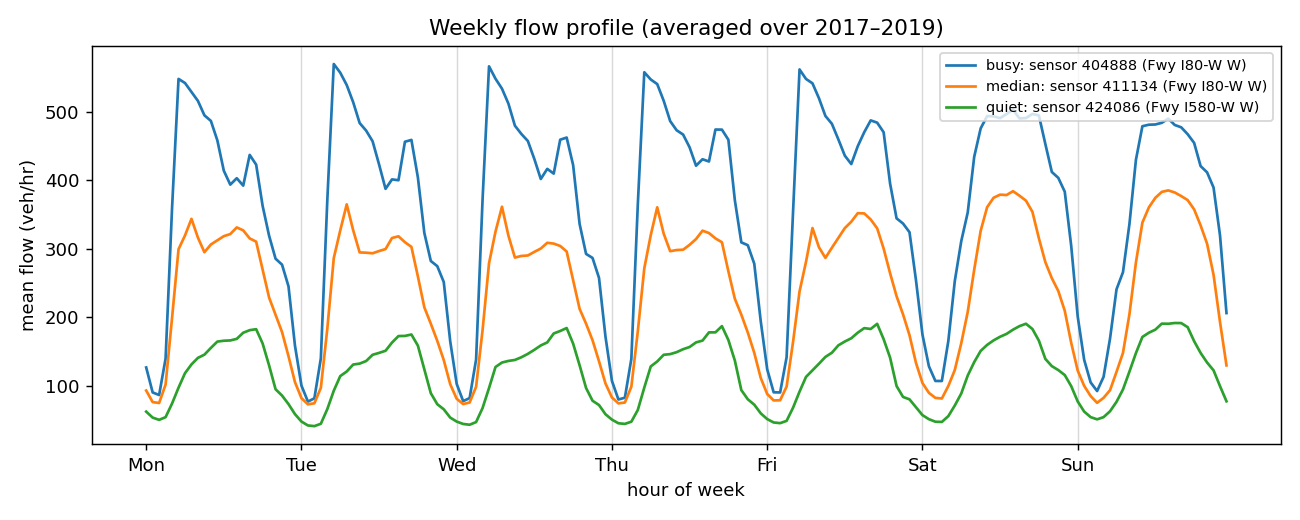
\includegraphics[width=0.92\linewidth]{fig1_weekly_profile.png}
\caption{Mean flow by hour-of-week for three sensors. The weekday commute
double-peak and the weekend single hump repeat with high regularity -- the
deterministic ``shape'' the rule exploits.}
\label{fig:profile}
\end{figure}

\subsection{Step 1 -- the seasonal baseline (last-4-weeks average)}

Predict each future hour by its recent average \emph{at the same hour of week}:
\begin{equation}
b_t \;=\; \frac{y_{t-168} + y_{t-336} + y_{t-504} + y_{t-672}}{4},
\end{equation}
that is, the mean of the same weekday-and-hour over the previous four weeks (the
lags $168,336,504,672$ are simply $1,2,3,4$ weeks in hours). Every term is at least
a week old, so at the forecast origin the \emph{entire} next week is computable from
data already in hand -- the rule is leakage-free for week-ahead use.

\paragraph{Worked example.} Forecast next \textbf{Wednesday 08:00} (a commute peak)
at a busy sensor. The last four Wednesdays at 08:00 read $540, 560, 535, 555\veh$
(oldest to newest). Then
\[
b = \tfrac14(540+560+535+555) = \mathbf{547.5}\veh.
\]

\subsection{Step 2 -- recency weighting (a one-parameter upgrade)}

When the level is drifting (slow growth, a seasonal transition), weight recent weeks
more. Use geometric weights $\propto \alpha^{0},\alpha^{1},\alpha^{2},\alpha^{3}$
with $\alpha \approx 0.8$, normalized to sum to one -- about
$(0.34, 0.27, 0.22, 0.17)$ from the most recent week to the oldest:
\begin{equation}
b_t^{\text{ewma}} \;=\; 0.34\,y_{t-168} \;+\; 0.27\,y_{t-336} \;+\; 0.22\,y_{t-504}
\;+\; 0.17\,y_{t-672}.
\end{equation}

\paragraph{Worked example (rising level).} If the last four same-hour values are
$500, 520, 540, 560\veh$ (oldest to newest), the flat average is $530$, while the
recency-weighted value is
\[
0.34(560)+0.27(540)+0.22(520)+0.17(500) = \mathbf{537.4}\veh,
\]
leaning toward the recent, higher values and so tracking the upward drift the flat
average lags. (In a flat period the two coincide.) Fitting the single decay
$\alpha$ on past data is the only ``training'' in the whole rule, and a fixed
$\alpha=0.8$ works well.

\subsection{Step 3 -- the holiday / calendar adjustment}

The baseline has one clear blind spot: \textbf{holidays}. To forecast the Fourth of
July it averages four \emph{ordinary} weeks and badly over-predicts, because a
holiday reshapes the day -- the morning commute largely disappears
(Figure~\ref{fig:holiday}). Holidays are only about $8\%$ of hours but contribute
roughly $23\%$ of the squared error, and they are \emph{known in advance} -- so we
correct them explicitly with a multiplicative factor.

For a given holiday and a given hour of the day, define the factor in words:
\begin{quote}
\emph{the factor is the average, over past occurrences of that holiday, of the
ratio (actual flow) / (baseline flow) at that hour of the day.}
\end{quote}
Concretely, if a holiday has occurred twice in the training data and at 17:00 its
flow was $0.70$ and $0.72$ times the baseline on those two days, the factor is
\begin{equation}
f \;=\; \frac{0.70 + 0.72}{2} \;=\; 0.71 .
\end{equation}
A factor below one means the holiday-hour runs below its ordinary-week level; the
adjusted forecast on special days is simply
\begin{equation}
\hat y_t \;=\; b_t^{\text{ewma}} \times f .
\end{equation}

\paragraph{Worked example.} Suppose the baseline for the Fourth of July at 17:00 is
$490\veh$ (from the four ordinary weeks before it) and the learned factor for
``Independence Day, 17:00'' is $0.71$. Then
\[
\hat y = 490 \times 0.71 = \mathbf{348}\veh,
\]
a $29\%$ correction exactly where the plain baseline fails.

\begin{figure}[H]\centering
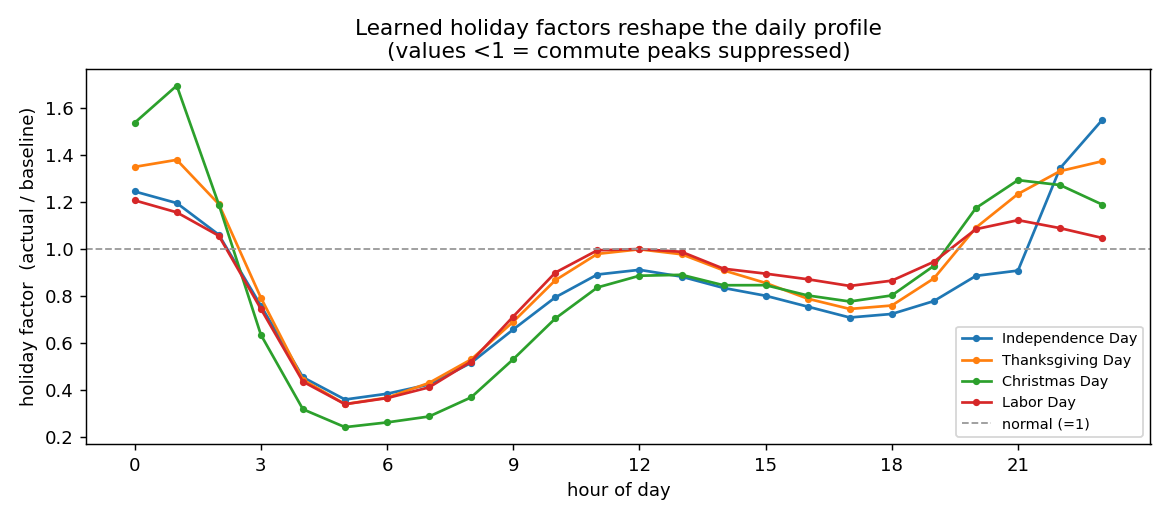
\includegraphics[width=0.9\linewidth]{fig6_holiday_shape.png}
\caption{Learned holiday factors by hour of day. Values below one crush the commute
peaks (mornings drop to $\sim$0.35--0.45); the late-evening values above one reflect
holiday-eve travel.}
\label{fig:holiday}
\end{figure}

\paragraph{Practicalities that matter.}
\begin{itemize}\itemsep2pt
\item \textbf{Multiplicative, not additive}: the holiday effect scales with the
  level, so a ratio transfers across busy and quiet weeks; a fixed offset does not.
\item \textbf{Per hour of day}: holidays reshape the daily profile, so the factor
  varies across the 24 hours (Figure~\ref{fig:holiday}).
\item \textbf{Pool across years} (and across sensors) to denoise the factor -- each
  holiday occurs only once a year.
\item \textbf{Include shoulder days}: the day before and after a holiday, and
  ``bridge'' days, each get their own factor.
\item \textbf{Known-ahead}: because holidays come from the calendar, the factor is
  available at any horizon -- no forecast of an input is required.
\end{itemize}

\subsection{The rule, in one line}

\begin{center}
\fbox{\begin{minipage}{0.92\linewidth}\centering\vspace{2pt}
\textbf{Forecast} $=$ (recency-weighted average of the same hour-of-week over the
last few weeks) $\times$ (holiday factor on special days, otherwise $1$).
\vspace{2pt}\end{minipage}}
\end{center}

\noindent
A worked holiday day, hour by hour, shows the two pieces combining:

\begin{table}[H]\centering
\caption{A holiday reshaped by the learned factor (illustrative values).}
\begin{tabular}{cccc}
\toprule
hour & baseline $b^{\text{ewma}}$ (\veh) & factor $f$ & forecast $\hat y$ (\veh) \\
\midrule
08:00 & 520 & 0.42 & 218 \\
12:00 & 430 & 0.96 & 413 \\
17:00 & 490 & 0.71 & 348 \\
22:00 & 240 & 1.30 & 312 \\
\bottomrule
\end{tabular}
\end{table}

\section{Why it is hard to beat}

\paragraph{Performance.} On a rolling-origin 2019 backtest (factors learned only
from 2017--18), the pieces stack cleanly:

\begin{table}[H]\centering
\caption{One-week-ahead accuracy, GBA flow, test 2019 (all 2{,}352 sensors).}
\begin{tabular}{lccc}
\toprule
Model & $R^2$ & RMSE (\veh) & RMSE on holiday hours \\
\midrule
Flat 4-week baseline        & 0.9404 & 40.14 & 66.96 \\
\;+ recency weighting (EWMA)& 0.9435 & 39.10 & 65.99 \\
\;+ holiday factor          & \textbf{0.9493} & \textbf{37.01} & \textbf{47.71} \\
\bottomrule
\end{tabular}
\end{table}

\noindent
The holiday factor cuts holiday-hour error by $29\%$ ($67\!\to\!48\veh$) and leaves
ordinary hours untouched; the weekly-aggregate MAPE is $3.55\%$.

\paragraph{It sits at the practical ceiling.} Fit the best possible structure
\emph{in-sample} on 2019 itself (perfect parameters, an upper bound): a static
hour-of-week mean reaches $R^2 = 0.938$, and adding an oracle holiday effect
$0.943$. Our \emph{out-of-sample} rule scores $0.949$ -- \emph{above} the in-sample
static oracle, because the recency weighting tracks within-year drift a fixed mean
cannot. The remaining $\sim$5\% of variance is dominated by irreducible,
incident-driven noise that no week-ahead model can recover.

\paragraph{Everything fancier failed to beat it.} We tried the usual escalations;
none added meaningful skill (Table~\ref{tab:tried}). The reason is structural: the
hour-of-week shape is deterministic and already captured, what little
autoregressive signal exists in the residual decays away over a one-week horizon,
and calendar/sensor features the baseline already encodes carry no new information.

\begin{table}[H]\centering
\caption{Attempts to beat the rule on endogenous information, and what they added.}
\label{tab:tried}
\begin{tabular}{>{\raggedright\arraybackslash}p{7.2cm}>{\raggedright\arraybackslash}p{7.6cm}}
\toprule
Attempt & Effect vs.\ the rule \\
\midrule
Autoregression on the residual (hourly lags)       & $\le +0.003\,R^2$; decays to $0$ by a week out \\
Autoregression on weekly-aggregate residual        & $\le +0.001\,R^2$ \\
Ridge / gradient boosting on calendar + sensor features & $\approx 0$ (high-cardinality features overfit) \\
Pooled panel AR (coefficients shared, $+$Fourier)  & worse than the rule \\
Global gradient boosting on the weekly panel       & worse than the rule \\
Cross-regional common factor (LA, San Diego)       & exists but is unforecastable (white in time) \\
\bottomrule
\end{tabular}
\end{table}

The through-line: on this problem, \textbf{a one- or two-parameter rule is at the
ceiling}, because the predictable part is a deterministic calendar pattern and the
rest is noise. Model complexity has nothing to feed on.

\section{Thoughts on how to improve it}

We do not think more sophisticated models of the \emph{same information} will help.
Genuine gains have to come from new information or a changed objective.

\begin{enumerate}\itemsep3pt
\item \textbf{Known-ahead exogenous signals.} The holiday factor works because
  holidays are calendar-known anomalies the baseline misses. The natural
  generalization is other \emph{known-ahead} events: scheduled sport/concerts and
  planned lane closures / roadwork. These are valid at any horizon (no forecast of
  the input needed). The caveat is granularity -- a stadium event is large but
  localized and brief, so it helps the few sensors near the venue at the day/hour
  level, not the network aggregate.
\item \textbf{Longer horizons and a longer record.} One week ahead is essentially
  solved; the open problem is multi-week, where a slowly-drifting \emph{level}
  governs the error. Modeling that level (trend, annual cycle) becomes worthwhile
  from about three to four weeks out, and learning slow multi-year structure needs
  more than three years of data.
\item \textbf{Distributional forecasts.} Everything above is a point forecast, but
  much operational value is in the tails -- the probability of severe congestion,
  calibrated intervals. The residual is heteroscedastic (heavy-tailed around peaks
  and incidents), so quantile or distributional methods add value for \emph{risk},
  not for the mean.
\item \textbf{Harder targets.} We forecast flow, which is highly seasonal. Speed is
  far noisier (a parallel check reached only $R^2 \approx 0.76$) and is a genuinely
  harder, more open problem.
\end{enumerate}

\noindent
The unifying lesson is simple: \textbf{complexity should follow information and
objective, not precede them.} For week-ahead flow, the information is a clean
calendar pattern and the objective is the mean -- so a calendar-adjusted seasonal
average is not just a baseline, it is close to the best one can do.

\paragraph{Reproducibility.} All numbers and figures come from the project's
\texttt{src/} scripts (the seasonal/EWMA/holiday models, the oracle-floor and
feature-merit analyses, and the pooled and cross-regional experiments), on the open
LargeST dataset.

\end{document}
